\datos{color}{}{}

\subsection{Pez robot \textit{UJI–CIRTESU}}

El pez robot desarrollado por el \textit{Interactive and Robotic Systems Laboratory} (\textit{IRS-Lab}) 
de la \textit{Universitat Jaume I} (\textit{UJI}), en colaboración con el grupo \textit{CIRTESU},
Figura \ref{pezrobot}, 
representa una plataforma biomimética diseñada para la exploración y monitorización en 
entornos submarinos. El sistema fue presentado en las \textit{Jornadas de Automática 2025}, 
donde recibió el premio al mejor trabajo en Automática Marina. Su diseño se inspira en la 
locomoción ondulatoria de los peces, integrando electrónica embarcada, sensores y un 
mecanismo de propulsión basado en aletas flexibles. \\

Sus usos principales incluyen la investigación en robótica submarina, el estudio de 
locomoción biomimética, la monitorización ambiental en puertos y zonas costeras, y la 
experimentación con sistemas de comunicación acústica entre robots marinos. El pez robot 
ha sido empleado en pruebas reales en el puerto de Castellón, donde interactuó con un 
robot de superficie mediante un enlace acústico de baja tasa. \\

La arquitectura del sistema sigue un modelo completamente centralizado y jerárquico. 
El robot submarino ejecuta únicamente el control de bajo nivel asociado al movimiento 
de las aletas y la estabilización, mientras que la planificación, supervisión y toma de 
decisiones se realizan en un ordenador externo situado en el robot de superficie. 
La comunicación entre ambos se establece mediante un módem acústico, lo que refuerza 
la estructura maestro–esclavo del sistema. El flujo de control sigue la secuencia clásica: 
sensado local $\rightarrow$ transmisión acústica $\rightarrow$ planificación en superficie 
$\rightarrow$ envío de comandos $\rightarrow$ acción. \\

\begin{wrapfigure}{r}{0.4\textwidth}
    \centering
    \vspace{-10pt}
    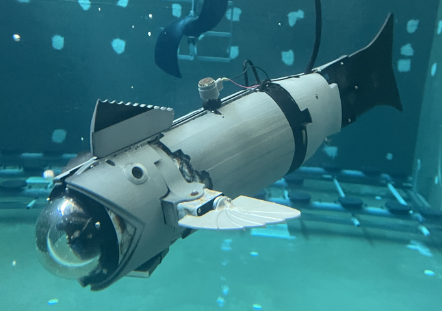
\includegraphics[width=0.36\textwidth]{Images/pez.png}
    \caption{Pez robot \textit{UJI–CIRTESU}.}
    \label{pezrobot}
    \vspace{-10pt}
\end{wrapfigure}

El método de locomoción se basa en una aleta de cola y dos laterales, todas accionadas por servomotores.
La aleta de cola genera un movimiento oscilatorio periódico. Este mecanismo produce una propulsión 
similar a la de los peces reales, permitiendo maniobrabilidad, eficiencia energética y 
movimientos suaves en el medio acuático. El diseño biomimético facilita la navegación en 
espacios reducidos y reduce el impacto ambiental respecto a los sistemas de hélice 
convencionales.

\subsection*{Referencias}

\cite{Puig2025FishRobot} \fullcite{Puig2025FishRobot}.\\
\cite{PortCastello2025PezRobot} \fullcite{PortCastello2025PezRobot}.
